\documentclass[../../../main.tex]{subfiles}
\begin{document}
Les graphes constituent un outil fondamental de modélisation d'ensembles structurés par des relations. Ils interviennent chaque fois qu'on étudie un ensemble de liaisons (orientés ou non) entre les éléments d'un ensemble d'objets. On trouve des graphes par exemple :
\begin{itemize}
	\item dans la modélisation d'un réseau (Internet, relations social, etc\dots)
	\item dans la modélisation de problèmes d'ordonnancement de tâches en recherche opérationnelle
	\item la modélisation de systèmes complexes par la représentation des passages d'un état à un autre
	\item en théorie des jeux pour la modélisation d'arbres d'évaluation\footnote{Un arbre est un graphe particulier.}
	\item en optimisation à la compilation en modélisant par un graphe les dépendances d'expressions d'un programme
	\item la représentation de modèles de théories
	\item etc\dots
\end{itemize}
Autant dire : un peu partout.

La recherche des algorithmes les plus efficaces pour réaliser les opérations de base sur les graphes constitue donc un objectif essentiel de l’algorithmique.

Les algorithmes décrits dans la suite ne sont pas exigés tels quels aux examens d'\textit{Algo/Prog} de l'ISMIN\footnote{Puisque n'est pas encore arrivée à l'ISMIN l'exigence tout court. Ou alors, ça fait longtemps qu'elle est partie voir ailleurs\dots}. Ils sont à connaître pour la culture. Il s'agit du minimum syndical des connaissances algorithmiques sur les graphes. Les connaître permet de se familiariser avec les bases pour avancer avec plus d'aisance à travers des propriétés moins simples.

\textbf{Remarque :} Il a été essayé de présenter chaque algorithme avec un maximum de rigueur sans pour autant être \textit{trop} formel. Le but est de donner une intuition bien-fondé du fonctionnement et de la correction des algorithmes. On justifie donc principalement ``avec les mains'' les algorithmes et l'intuition que l'on peut avoir de leur fonctionnement. On peut trouver un cours bien plus formel et absolument rigoureux en bibliographie \cite{ENSGraphes}.
\subsection{Définition et représentations}
De nombreuses définitions sont nécessaires pour discuter efficacement des graphes. C'est un gros sujet, qu'on ne traite que pour une infime partie.
\definition{Graphe orienté} {
	On définit un \textit{graphe orienté} $G$ (ou simplement \textit{graphe}) comme un couple $(S, A)$ où :
	\begin{itemize}
		\item $S$ est un ensemble fini de \textit{sommets}\footnote{C'est-à-dire en bijection avec un sous-ensemble de $\mathbb{N}$} du graphe.\newline
		On considère sans perte de généralité $S = \{0, \dots, n-1\}$, où $n = |S|\in\mathbb{N}$ le nombre de sommets de $G$ est applé son \textit{ordre}.
		\item $A\subseteq S\times S$ est l'ensemble des \textit{arcs} du graphe, c'est-à-dire des liaisons orientés entre les sommets.
	\end{itemize}
	Soient $u, v\in S$. On note $u\rightarrow v$ pour dire qu'il existe un arc de $u$ vers $v$ dans $G$, c'est-à-dire que $(u, v)\in A$. On dit alors que :
	\begin{itemize}
		\item $u$ est un \textit{prédécesseur} de $v$
		\item $v$ est un \textit{successeur} de $u$
	\end{itemize}
}
\textbf{Exemple :} Ci-dessous un dessin d'un graphe $G = (S, A)$ d'ordre $5$ avec : 
\begin{itemize}
	\item $S = \{0, 1, 2, 3, 4\}$
	\item $A = \{(0, 1), (1, 0), (1, 3), (2, 4), (2, 3), (3, 2), (4, 0), (4, 1), (4, 3)\}$
\end{itemize}
\begin{center}
	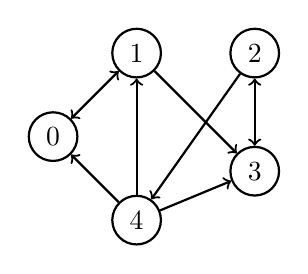
\begin{tikzpicture}[node distance={15mm}, thick, main/.style = {draw, circle}] 
	% Sommets :
	\node[main] (0) {$0$}; 
	\node[main] (1) [above right of=0] {$1$};
	\node[main] (2) [right of=1] {$2$};
	\node[main] (3) [below of=2] {$3$};
	\node[main] (4) [below right of=0] {$4$};
	% Arêtes
	\draw[->] (2) -- (4);
	\draw[->] (4) -- (0);
	\draw[->] (4) -- (1);
	\draw[->] (4) -- (3);
	\draw[<->] (2) -- (3);
	\draw[<->] (0) -- (1);
	\draw[->] (1) -- (3);
	\end{tikzpicture}
	\captionof{figure}{Graphe orienté}\label{graph:oriented}
\end{center}
\definition{Graphe non orienté} {
	Un graphe $G = (S, A)$ est dit \textit{non orienté} si : $$\forall u,v\in S,(u, v)\in A \Rightarrow (v, u)\in A$$
	On peut alors simplifier par $A\subseteq \{\{u, v\}\ |\ u, v\in S\}$. Les éléments $\{u, v\}\in A$ sont appelés les \textit{arêtes} de $G$.\newline

	Soient $u, v\in S$. On note $u -- v$ pour dire qu'il existe une arête entre $u$ et $v$ dans $G$, c'est-à-dire que $\{u, v\}\in A$. On dit alors que $u$ et $v$ sont \textit{adjacents} ou \textit{voisins}.
}
\textbf{Remarque :} on peut toujours voir un graphe non orienté $G = (S, A)$ comme un graphe orienté $G = (S, \{(u, v), (v, u)\ |\ \{u, v\}\in A\})$

\textbf{Exemple :} Ci-dessous un dessin d'un graphe $G = (S, A)$ d'ordre $8$ avec :
\begin{itemize}
	\item $S = \{0, 1, 2, 3, 4, 5, 6, 7\}$
	\item $A = \{\{0, 4\}, \{0, 1\}, \{2, 3\}, \{3, 5\}, \{3, 6\}, \{5, 7\}, \{6, 7\}\}$
\end{itemize}
\begin{center}
	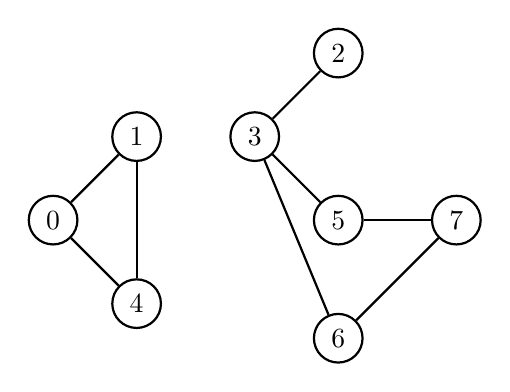
\begin{tikzpicture}[node distance={15mm}, thick, main/.style = {draw, circle}] 
	% Sommets :
	\node[main] (0) {$0$}; 
	\node[main] (1) [above right of=0] {$1$};
	\node[main] (3) [right of=1] {$3$};
	\node[main] (2) [above right of=3] {$2$};
	\node[main] (5) [below right of=3] {$5$};
	\node[main] (6) [below of=5] {$6$};
	\node[main] (4) [below right of=0] {$4$};
	\node[main] (7) [right of=5] {$7$};
	% Arêtes
	\draw (3) -- (6);
	\draw (4) -- (1);
	\draw (4) -- (0);
	\draw (2) -- (3);
	\draw (1) -- (0);
	\draw (3) -- (5);
	\draw (6) -- (7);
	\draw (5) -- (7);
	\end{tikzpicture} 
	\captionof{figure}{Graphe non orienté}\label{graph:non_oriented}
\end{center}
\definition{Degré entrant d'un sommet}{
	Soit $G = (S, A)$ un graphe (orienté). Le degré \textit{entrant} d'un sommet $u\in S$ est :
	$$d^-(u) = Card(\{(v, u)\in A\ |\ v\in S\})$$
	C'est le nombre d'arcs qui arrivent à $u$, c'est-à-dire le nombre de prédécesseurs de $u$ dans $G$
}
\definition{Degré sortant d'un sommet}{
	Soit $G = (S, A)$ un graphe (orienté). Le degré \textit{sortant} d'un sommet $u\in S$ est :
	$$d^+(u) = Card(\{(u, v)\in A\ |\ v\in S\})$$
	C'est le nombre d'arcs qui partent de $u$, c'est-à-dire le nombre de successeurs de $u$ dans $G$
}
\definition{Degré d'un sommet}{
	Soit $G = (S, A)$ un graphe (orienté). Le degré d'un sommet $u\in S$ est la somme du degré entrant et du degré sortant de $u$. On note :
	$$d(u) = d^-(u) + d^+(u)$$
}
\textbf{Exemple :} Dans le graphe suivant :
\begin{center}
	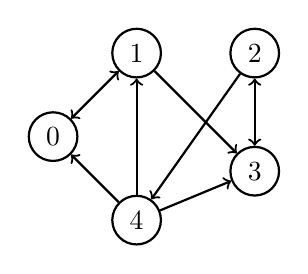
\begin{tikzpicture}[node distance={15mm}, thick, main/.style = {draw, circle}] 
	% Sommets :
	\node[main] (0) {$0$}; 
	\node[main] (1) [above right of=0] {$1$};
	\node[main] (2) [right of=1] {$2$};
	\node[main] (3) [below of=2] {$3$};
	\node[main] (4) [below right of=0] {$4$};
	% Arêtes
	\draw[->] (2) -- (4);
	\draw[->] (4) -- (0);
	\draw[->] (4) -- (1);
	\draw[->] (4) -- (3);
	\draw[<->] (2) -- (3);
	\draw[<->] (0) -- (1);
	\draw[->] (1) -- (3);
	\end{tikzpicture} 
\end{center}
On a $d^+(3) = 1$ et $d^-(3) = 3$ donc $d(3) = d^+(3) + d^-(3) = 4$.
\subsection{Signature du type abstrait}
\label{sub:signature_du_type_abstrait_graphe}
Avant de présenter les représentations standards en mémoire  des graphes, on présente une signature minimale des routines de manipulation des graphes. Ces routines permettront de mettre en évidence quelles sont les opérations fondamentales sur les graphes qui seront utiles pour la quasi-totalité des algorithmes dans la suite.

\textit{Graphe\textless Sommet\textgreater} utilise \textit{Liste\textless Sommet\textgreater}, \textit{Sommet}, \textit{Entier} :
\begin{itemize}
	\item $creer(Graphe, Entier:n)\rightarrow Graphe$ renvoie un graphe d'ordre $n$ sans arêtes.
	\item $degre(Graphe, Sommet:s)\rightarrow Entier$ renvoie $d(s)$ le degré de $s$
	\item $succ(Graphe, Sommet:s)\rightarrow \textit{Liste\textless Sommet\textgreater}$ renvoie la liste des successeurs de $s$
	\item $prec(Graphe, Sommet:s)\rightarrow \textit{Liste\textless Sommet\textgreater}$ renvoie la liste des prédécesseurs de $s$
	\item $ajouter\_sommet(Graphe:G)\rightarrow Graphe$ renvoie pour $G = (S, A)$ originellement d'ordre $n$ le graphe $G'=(S\cup\{n\}, A)$ d'ordre $(n+1)$
	\item $supprimer\_sommet(Graphe:G, Sommet:s)\rightarrow Graphe$ renvoie pour $G = (S, A)$ originellement d'ordre $n$ le graphe $G'=(S\setminus\{s\}, A)$ d'ordre $(n+1)$\footnote{On remarque que $S = \{0, \dots, s-1, s+1, \dots, n\}$ puisque le sommet est quelconque dans $S$.}
	\item $ajouter\_arc(Graphe:G, Sommet:u, Sommet:v)\rightarrow Graphe$ renvoie pour $G = (S, A)$ le graphe $G' = (S, A\cup\{(u, v)\})$ résultant de l'ajout de l'arc $(u, v)$
	\item $supprimer\_arc(Graphe:G, Sommet:u, Sommet:v)\rightarrow Graphee$ renvoie pour $G = (S, A)$ le graphe $G' = (S, A\setminus\{(u, v)\})$ résultant du retrait de l'arc $(u, v)$
\end{itemize}
\textbf{Remarque 1 :} La signature ci-dessus ne préjuge en rien du type $Sommet$, bien qu'on puisse le plus souvent l'assimiler à $Entier$ lors de l'implantation.

\textbf{Remarque 2 :} C'est l'efficacité des routines $succ$ et $prec$ qui garantit l'efficacité du parcours des sommets d'un graphe, et donc de la plupart des manipulations de celui-ci. La routine $succ$ est prioritaire sur $prec$ dans la plupart des cas d'utilisation.
\subsection{Représentations}
\label{sub:representations_graphe}
On peut représenter d'au moins trois façons standard un graphe en mémoire :
\begin{itemize}
	\item par matrice d'adjacence
	\item par liste de successeurs
	\item \textit{\tiny(par matrice d'incidence, qu'on ne présentera pas ici de par son aspect particulièrement mineur dans la pratique comme dans la théorie)}
\end{itemize}
\subsubsection{Matrice d'adjacence}
On peut représenter un graphe $G = (S, A)$ comme une matrice $M\in\mathcal{M}_{|S|}(\mathcal{B})$. On a alors :
$$\forall u, v\in S,
M_{u, v} = \left\{\begin{array}{lcl}
\textit{Vrai} & \text{si} & (u, v)\in A\\
\textit{Faux} & \text{si} & (u, v)\not\in A
\end{array}\right.
$$
\textbf{Exemple :} avec $\textit{Vrai}\equiv 1$ et $\textit{Faux}\equiv 0$

\begin{minipage}{0.5\textwidth}
	\begin{center}
		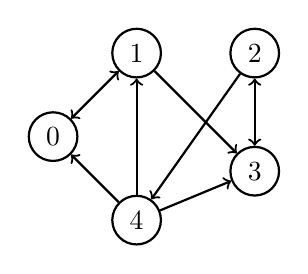
\begin{tikzpicture}[node distance={15mm}, thick, main/.style = {draw, circle}] 
		% Sommets :
		\node[main] (0) {$0$}; 
		\node[main] (1) [above right of=0] {$1$};
		\node[main] (2) [right of=1] {$2$};
		\node[main] (3) [below of=2] {$3$};
		\node[main] (4) [below right of=0] {$4$};
		% Arêtes
		\draw[->] (2) -- (4);
		\draw[->] (4) -- (0);
		\draw[->] (4) -- (1);
		\draw[->] (4) -- (3);
		\draw[<->] (2) -- (3);
		\draw[<->] (0) -- (1);
		\draw[->] (1) -- (3);
		\end{tikzpicture}
	\end{center}
\end{minipage}
\begin{minipage}{0.5\textwidth}
$$
\begin{pmatrix}
	0 & 1 & 0 & 0 & 0 \\
	1 & 0 & 0 & 1 & 0 \\
	0 & 0 & 0 & 1 & 1 \\
	0 & 0 & 1 & 0 & 0 \\
	1 & 1 & 0 & 1 & 0
\end{pmatrix}
$$
\end{minipage}
\underline{\textbf{Complexité spatiale :}}\newline
Cette représentation est de complexité spatiale en $\Theta(|S|^2)$.

\underline{\textbf{Complexités temporelles des routines de parcours :}}\newline
On peut déduire, pour tout $u\in S$
\begin{itemize}
	\item la liste des successeurs de $u$ par le parcours de la $u^e$ ligne de $M$ (en $\Theta(|S|)$)
	\item la liste des prédécesseurs de $u$ par le parcours de la $u^e$ colonne de $M$ (en $\Theta(|S|)$)
\end{itemize}
\textit{idem} pour les calculs de $d^+(u)$ et $d^-(u)$

On va voir avec la représentation par liste de successeurs que le calcul des successeurs est plus rapide mais que le calcul des prédécesseurs est substantiellement plus long (dans le pire cas, en $O(|S|log_2(|S|))$ si la liste est triée, $O(|S|^2)$ sinon)
\subsubsection{Liste de successeurs}
Si un graphe $G = (S, A)$ contient peu d'arêtes, la matrice d'adjacence représentative de $G$ est creuse. On observe d'abord que la mémoire est gaspillée par le stockage d'une grande quantitée de $0$ inutiles, d'autre part que le calcul du degré sortant/des successeurs d'un sommet de $G$ n'est pas optimisé puisqu'il faut prendre en considération beaucoup d'absence d'arêtes, qu'on sait absentes si on sait la matrice creuse.

L'idée de la représentation d'un graphe par listes de successeurs est d'associer à chaque sommet $u\in S$ la liste de ses successeurs $succ(u)$ dans $G$. On peut facilement se convaincre que stocker ainsi les successeurs de tous les sommets permet bien de stocker toutes les arêtes, puisque chaque arête part d'un sommet pour \textit{lui en faire succéder} un autre.

\textbf{Exemple :}

\begin{minipage}{0.5\textwidth}
	\begin{center}
		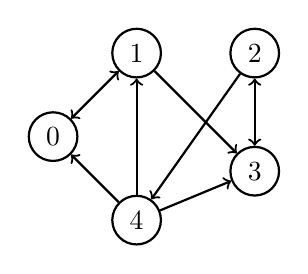
\begin{tikzpicture}[node distance={15mm}, thick, main/.style = {draw, circle}] 
		% Sommets :
		\node[main] (0) {$0$}; 
		\node[main] (1) [above right of=0] {$1$};
		\node[main] (2) [right of=1] {$2$};
		\node[main] (3) [below of=2] {$3$};
		\node[main] (4) [below right of=0] {$4$};
		% Arêtes
		\draw[->] (2) -- (4);
		\draw[->] (4) -- (0);
		\draw[->] (4) -- (1);
		\draw[->] (4) -- (3);
		\draw[<->] (2) -- (3);
		\draw[<->] (0) -- (1);
		\draw[->] (1) -- (3);
		\end{tikzpicture}
	\end{center}
\end{minipage}
\begin{minipage}{0.5\textwidth}
$$
\begin{array}{lcl}
0 & : & [1] \\
1 & : & [0, 3] \\
2 & : & [4, 3] \\
3 & : & [2] \\
4 & : & [0, 3, 1] \\
\end{array}
$$
\end{minipage}

\textbf{Remarque :} les listes de successeurs ne sont pas nécessairement triées. Toutefois, leur tri peut être un propriété appréciable pour l'efficacité de certaines routines de manipulation.
\subsection{Propriétés}
\definition{Chemin élémentaire} {
	Soit $G = (S, A)$. Soient deux sommets $u, v\in S$. Un chemin $\gamma$ de $u$ à $v$ est élémentaire si tous les sommets de $\gamma$ sont différents. Aucun ne se répète.
}
\lemma{König} Soit $G = (S, A)$. Soient deux sommets $u, v\in S$. Il existe un chemin de longueur minimal entre $u$ et $v$. Ce chemin est élémentaire.

\textbf{Démonstration (un peu avec les mains\footnote{Mais à un concours de sortie de prépa, ça passe crème.}) :} Un chemin $\gamma$ de longueur minimal existe nécessairement car le graphe est fini, donc son nombre de chemins entre $u$ et $v$ aussi et ces chemins sont ordonnés totalement par la relation ``est plus court que''. Si un sommet $w$ se répète dans $\gamma$, alors il existe un sous-chemin $w\rightarrow \dots \rightarrow w$ dans $\gamma$. On peut le supprimer, et la répétition avec.
\subsection{Parcours en profondeur et en largeur}
\subsubsection{Principe et exemples}
\definition{Parcours} {
	Un parcours est une liste de tous les sommets d'un graphe $G$ $L = [s_1, \dots, s_n]$ telle que pour tout $j\in\{2, \dots, n\}$, il existe $i < j$ tel que $s_i\rightarrow s_j$.\newline

	En d'autres termes, lors d'un parcours de graphe, un sommet (autre que le premier) ne peut être visité que s'il est le successeur d'un sommet déjà visité. Sinon, ce n'est pas un parcours, c'est autre chose.	
}
La différence entre un parcours en profondeur et un parcours en largeur tient donc dans le choix de l'ordre de visite.
\definition{Parcours partiel} {
	Un parcours partiel est une liste $L = [s_1, \dots, s_k]$ avec $k \leq n$ de sommets tous différents de $G$ telle que pour tout $j\in\{2, \dots, k\}$, il existe $i < j$ tel que $s_i\rightarrow s_j$.\newline

	En d'autres termes, c'est un parcours pas fini d'un graphe. $L_n$ est un parcours complet (on a visité tous les $n$ sommets).
}
\textbf{Remarque :} À tout moment d'un parcours de graphe, certains sommets sont visités et d'autres ne le sont pas. Si tous les sommets sont visités, c'est que le parcours est fini. En particulier, cela signifie que tant que le parcours n'est pas fini, certains sommets ont des successeurs non visités.
\definition{Sommet ouvert} {
	Un sommet d'un parcours partiel $L_k$ est \textit{ouvert} s'il a au moins un successeur qui n'apparaît pas dans $L_k$, c'est-à-dire qui n'est pas encore visité.
}
\definition{Sommet fermé} {
	Un sommet d'un parcours partiel $L_k$ est \textit{fermé} si tout ses successeurs sont dans $L_k$, c'est-à-dire qui sont tous déjà visités.
}
\definition{Sommet découvert} {
	On appelle \textit{sommet découvert} par un parcours $L_k$ un sommet non visité (= pas dans $L_k$) qui est successeur d'un sommet visité (= dans $L_k$).
}
On observe deux choses :
\begin{itemize}
	\item le dernier sommet ouvert d'un parcours partiel est le plus récent sommet visité qui ait des successeurs non visités.
	\item le premier sommet ouvert d'un parcours partiel est le plus ancien sommet visité qui ait des successeurs non visités.
\end{itemize}
D'où deux choix qui apparaissent clairement :
\begin{enumerate}
	\item à chaque visite, choisir un successeur du plus récent sommet visité ouvert $\Rightarrow$ parcours en profondeur
	\item à chaque visite, choisir un successeur du plus ancien sommet visité ouvert $\Rightarrow$ parcours en largeur
\end{enumerate}
La définition de chacun des deux types de parcours est ainsi donné, en itérant le choix ci-dessus jusqu'à avoir parcouru tout le graphe. Maintenant, il s'agit de construire une intuition, c'est-à-dire de comprendre pourquoi ces parcours sont appelés \textit{en profondeur} et \textit{en largeur}. On s'occupera après de clarifier un algorithme pour chaque cas.

Dans les deux exemples qui suivent, on colorie :
\begin{itemize}
	\item en vert les sommets visités
	\item en gris les sommets découverts
	\item en bleu le sommet visité ouvert :
	\begin{itemize}
		\item le plus récent dans le cas du parcours en profondeur
		\item le plus ancien dans le cas du parcours en largeur
	\end{itemize}
\end{itemize}
Dans les deux cas, on parcours le graphe non orienté\footnote{Pour simplifier. Un graphe orienté, y a plein de cas bizarres de connexité, c'est plus chiant à lire.} suivant :
\begin{center}
		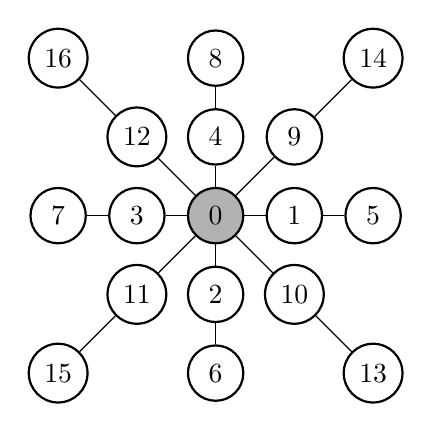
\begin{tikzpicture}
		[node distance={10mm},
		main/.style = {circle, draw, thick, 
                      minimum size=2em}] 
		% Sommets :
		\node[main, fill=black!30!white] (0) {$0$}; 
		\node[main] (1) [right of=0] {$1$};
		\node[main] (2) [below of=0] {$2$};
		\node[main] (3) [left of=0] {$3$};
		\node[main] (4) [above of=0] {$4$}; 
		\node[main] (5) [right of=1] {$5$};
		\node[main] (6) [below of=2] {$6$};
		\node[main] (7) [left of=3] {$7$};
		\node[main] (8) [above of=4] {$8$};
		\node[main] (9) [right of=4] {$9$};
		\node[main] (10) [right of=2] {$10$};
		\node[main] (11) [left of=2] {$11$};
		\node[main] (12) [left of=4] {$12$};
		\node[main] (13) [right of=6, xshift=10mm] {$13$};
		\node[main] (14) [right of=8, xshift=10mm] {$14$};
		\node[main] (15) [left of=6, xshift=-10mm] {$15$};
		\node[main] (16) [left of=8, xshift=-10mm] {$16$};
		% Arêtes
		\draw (0) -- (1);
		\draw (0) -- (10);
		\draw (0) -- (2);
		\draw (0) -- (11);
		\draw (0) -- (3);
		\draw (0) -- (12);
		\draw (0) -- (4);
		\draw (0) -- (9);

		\draw (1) -- (5);
		\draw (10) -- (13);
		\draw (4) -- (8);
		\draw (9) -- (14);
		\draw (2) -- (6);
		\draw (11) -- (15);
		\draw (3) -- (7);
		\draw (12) -- (16);
		\end{tikzpicture}
	\end{center}
Le premier sommet est donc à chaque fois $0$ puisqu'il s'agit du premier qu'on \textit{marque} comme découvert initialement et qui est donc le seul à pouvoir être visité.

\textbf{Exemple 1 (parcours en profondeur) :} On visite $0$. Donc $L_1 = [0]$ Les sommets découverts du parcours partiel $L_0$ sont les successeurs non visités des sommets de $L_0$, donc ici :
\begin{center}
		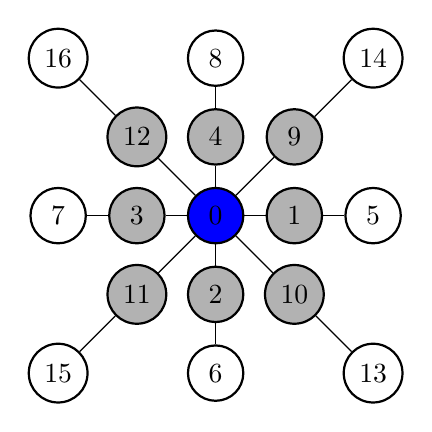
\begin{tikzpicture}
		[node distance={10mm},
		main/.style = {circle, draw, thick, 
                      minimum size=2em}] 
		% Sommets :
		\node[main, fill=blue] (0) {$0$}; 
		\node[main, fill=black!30!white] (1) [right of=0] {$1$};
		\node[main, fill=black!30!white] (2) [below of=0] {$2$};
		\node[main, fill=black!30!white] (3) [left of=0] {$3$};
		\node[main, fill=black!30!white] (4) [above of=0] {$4$}; 
		\node[main] (5) [right of=1] {$5$};
		\node[main] (6) [below of=2] {$6$};
		\node[main] (7) [left of=3] {$7$};
		\node[main] (8) [above of=4] {$8$};
		\node[main, fill=black!30!white] (9) [right of=4] {$9$};
		\node[main, fill=black!30!white] (10) [right of=2] {$10$};
		\node[main, fill=black!30!white] (11) [left of=2] {$11$};
		\node[main, fill=black!30!white] (12) [left of=4] {$12$};
		\node[main] (13) [right of=6, xshift=10mm] {$13$};
		\node[main] (14) [right of=8, xshift=10mm] {$14$};
		\node[main] (15) [left of=6, xshift=-10mm] {$15$};
		\node[main] (16) [left of=8, xshift=-10mm] {$16$};
		% Arêtes
		\draw (0) -- (1);
		\draw (0) -- (10);
		\draw (0) -- (2);
		\draw (0) -- (11);
		\draw (0) -- (3);
		\draw (0) -- (12);
		\draw (0) -- (4);
		\draw (0) -- (9);

		\draw (1) -- (5);
		\draw (10) -- (13);
		\draw (4) -- (8);
		\draw (9) -- (14);
		\draw (2) -- (6);
		\draw (11) -- (15);
		\draw (3) -- (7);
		\draw (12) -- (16);
		\end{tikzpicture}
	\end{center}
	On visite ensuite un successeur du plus récent sommet visité ouvert, \textit{i.e.} qui a encore des successeurs non visités. Comme $L_1$ ne contient que $0$, il suffit de choisir arbitrairement un successeur de $0$\footnote{On pourra choisir par exemple le premier découvert. Sachant que l'ordre de découverte est arbitraire (dépend de l'implantation), c'est pareil.} comme $4$ par exemple\footnote{\textit{Why not}.} :
	\begin{center}
		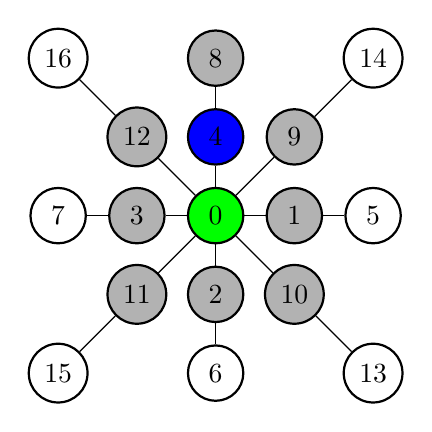
\begin{tikzpicture}
		[node distance={10mm},
		main/.style = {circle, draw, thick, 
                      minimum size=2em}] 
		% Sommets :
		\node[main, fill=green] (0) {$0$}; 
		\node[main, fill=black!30!white] (1) [right of=0] {$1$};
		\node[main, fill=black!30!white] (2) [below of=0] {$2$};
		\node[main, fill=black!30!white] (3) [left of=0] {$3$};
		\node[main, fill=blue] (4) [above of=0] {$4$}; 
		\node[main] (5) [right of=1] {$5$};
		\node[main] (6) [below of=2] {$6$};
		\node[main] (7) [left of=3] {$7$};
		\node[main, fill=black!30!white] (8) [above of=4] {$8$};
		\node[main, fill=black!30!white] (9) [right of=4] {$9$};
		\node[main, fill=black!30!white] (10) [right of=2] {$10$};
		\node[main, fill=black!30!white] (11) [left of=2] {$11$};
		\node[main, fill=black!30!white] (12) [left of=4] {$12$};
		\node[main] (13) [right of=6, xshift=10mm] {$13$};
		\node[main] (14) [right of=8, xshift=10mm] {$14$};
		\node[main] (15) [left of=6, xshift=-10mm] {$15$};
		\node[main] (16) [left of=8, xshift=-10mm] {$16$};
		% Arêtes
		\draw (0) -- (1);
		\draw (0) -- (10);
		\draw (0) -- (2);
		\draw (0) -- (11);
		\draw (0) -- (3);
		\draw (0) -- (12);
		\draw (0) -- (4);
		\draw (0) -- (9);

		\draw (1) -- (5);
		\draw (10) -- (13);
		\draw (4) -- (8);
		\draw (9) -- (14);
		\draw (2) -- (6);
		\draw (11) -- (15);
		\draw (3) -- (7);
		\draw (12) -- (16);
		\end{tikzpicture}
	\end{center}
	On a alors le parcours partiel $L_2 = [0, 4]$. Comme $4$ est ouvert, c'est le sommet ouvert le plus récent de $L_2$. On choisit un de ses successeurs \textit{non visité} (donc pas $0$), c'est-à-dire nécessairement $8$ :
	\begin{center}
		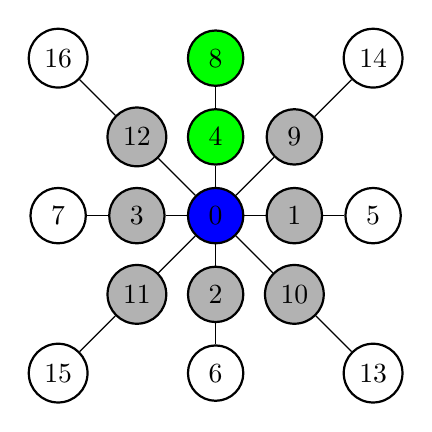
\begin{tikzpicture}
		[node distance={10mm},
		main/.style = {circle, draw, thick, 
                      minimum size=2em}] 
		% Sommets :
		\node[main, fill=blue] (0) {$0$}; 
		\node[main, fill=black!30!white] (1) [right of=0] {$1$};
		\node[main, fill=black!30!white] (2) [below of=0] {$2$};
		\node[main, fill=black!30!white] (3) [left of=0] {$3$};
		\node[main, fill=green] (4) [above of=0] {$4$}; 
		\node[main] (5) [right of=1] {$5$};
		\node[main] (6) [below of=2] {$6$};
		\node[main] (7) [left of=3] {$7$};
		\node[main, fill=green] (8) [above of=4] {$8$};
		\node[main, fill=black!30!white] (9) [right of=4] {$9$};
		\node[main, fill=black!30!white] (10) [right of=2] {$10$};
		\node[main, fill=black!30!white] (11) [left of=2] {$11$};
		\node[main, fill=black!30!white] (12) [left of=4] {$12$};
		\node[main] (13) [right of=6, xshift=10mm] {$13$};
		\node[main] (14) [right of=8, xshift=10mm] {$14$};
		\node[main] (15) [left of=6, xshift=-10mm] {$15$};
		\node[main] (16) [left of=8, xshift=-10mm] {$16$};
		% Arêtes
		\draw (0) -- (1);
		\draw (0) -- (10);
		\draw (0) -- (2);
		\draw (0) -- (11);
		\draw (0) -- (3);
		\draw (0) -- (12);
		\draw (0) -- (4);
		\draw (0) -- (9);

		\draw (1) -- (5);
		\draw (10) -- (13);
		\draw (4) -- (8);
		\draw (9) -- (14);
		\draw (2) -- (6);
		\draw (11) -- (15);
		\draw (3) -- (7);
		\draw (12) -- (16);
		\end{tikzpicture}
	\end{center}
	On a alors le parcours partiel $L_3 = [0, 4, 8]$. Comme $4$ et $8$ sont fermés, $0$ redevient le sommet ouvert visité le plus récemment. On visite alors un des successeurs non visité de $0$, donc un de ses successeurs différent de $4$. L'exécution est alors similaire à la visite de $4$ et $8$. On itère jusqu'à avoir parcouru tous les sommets du graphe.

	\textbf{Conclusion sur le parcours en profondeur :} le parcours va aller le plus loin possible puisqu'il choisi toujours les successeurs du sommet ouvert le plus récent. Il va \textit{le plus profond possible}\footnote{??? WTF} jusqu'à ne plus pouvoir aller plus loin. Il revient alors à l'ex. plus ancien sommet ouvert par la fermeture des sommets plus récents.\newline
	Un parcours final peut alors être $L = [0, 4, 8, 9, 14, 1, 5, 10, 13, 3, 7, 12, 16, 11, 15, 2, 6]$

	\textbf{Exemple 2 (parcours en largeur) :} on visite $0$. Donc $L_1 = [0]$ Les sommets découverts du parcours partiel $L_0$ sont les successeurs non visités des sommets de $L_0$, donc ici :
\begin{center}
		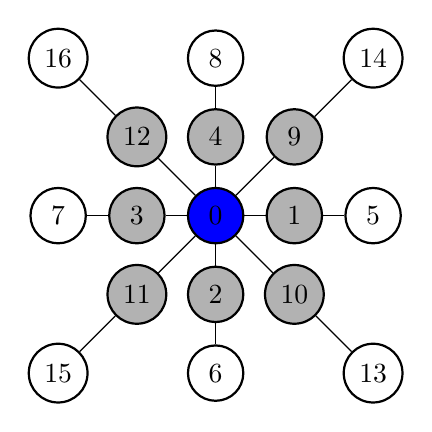
\begin{tikzpicture}
		[node distance={10mm},
		main/.style = {circle, draw, thick, 
                      minimum size=2em}] 
		% Sommets :
		\node[main, fill=blue] (0) {$0$}; 
		\node[main, fill=black!30!white] (1) [right of=0] {$1$};
		\node[main, fill=black!30!white] (2) [below of=0] {$2$};
		\node[main, fill=black!30!white] (3) [left of=0] {$3$};
		\node[main, fill=black!30!white] (4) [above of=0] {$4$}; 
		\node[main] (5) [right of=1] {$5$};
		\node[main] (6) [below of=2] {$6$};
		\node[main] (7) [left of=3] {$7$};
		\node[main] (8) [above of=4] {$8$};
		\node[main, fill=black!30!white] (9) [right of=4] {$9$};
		\node[main, fill=black!30!white] (10) [right of=2] {$10$};
		\node[main, fill=black!30!white] (11) [left of=2] {$11$};
		\node[main, fill=black!30!white] (12) [left of=4] {$12$};
		\node[main] (13) [right of=6, xshift=10mm] {$13$};
		\node[main] (14) [right of=8, xshift=10mm] {$14$};
		\node[main] (15) [left of=6, xshift=-10mm] {$15$};
		\node[main] (16) [left of=8, xshift=-10mm] {$16$};
		% Arêtes
		\draw (0) -- (1);
		\draw (0) -- (10);
		\draw (0) -- (2);
		\draw (0) -- (11);
		\draw (0) -- (3);
		\draw (0) -- (12);
		\draw (0) -- (4);
		\draw (0) -- (9);

		\draw (1) -- (5);
		\draw (10) -- (13);
		\draw (4) -- (8);
		\draw (9) -- (14);
		\draw (2) -- (6);
		\draw (11) -- (15);
		\draw (3) -- (7);
		\draw (12) -- (16);
		\end{tikzpicture}
	\end{center}
	On visite ensuite un successeur du plus ancien sommet visité ouvert, \textit{i.e.} qui a encore des successeurs non visités. Comme $L_1$ ne contient que $0$, il suffit de choisir arbitrairement un successeur de $0$\footnote{Voir la note de l'exemple de parcours en profondeur.} comme $4$ par exemple\footnote{\textit{Why not (again)}.} :
	\begin{center}
		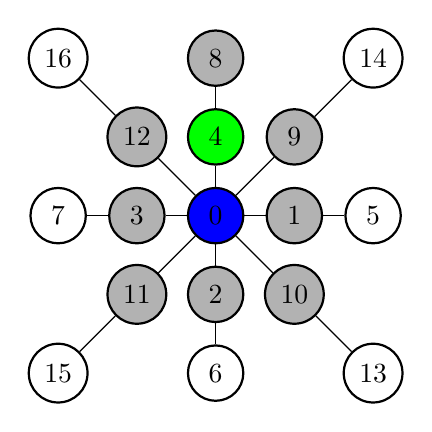
\begin{tikzpicture}
		[node distance={10mm},
		main/.style = {circle, draw, thick, 
                      minimum size=2em}] 
		% Sommets :
		\node[main, fill=blue] (0) {$0$}; 
		\node[main, fill=black!30!white] (1) [right of=0] {$1$};
		\node[main, fill=black!30!white] (2) [below of=0] {$2$};
		\node[main, fill=black!30!white] (3) [left of=0] {$3$};
		\node[main, fill=green] (4) [above of=0] {$4$}; 
		\node[main] (5) [right of=1] {$5$};
		\node[main] (6) [below of=2] {$6$};
		\node[main] (7) [left of=3] {$7$};
		\node[main, fill=black!30!white] (8) [above of=4] {$8$};
		\node[main, fill=black!30!white] (9) [right of=4] {$9$};
		\node[main, fill=black!30!white] (10) [right of=2] {$10$};
		\node[main, fill=black!30!white] (11) [left of=2] {$11$};
		\node[main, fill=black!30!white] (12) [left of=4] {$12$};
		\node[main] (13) [right of=6, xshift=10mm] {$13$};
		\node[main] (14) [right of=8, xshift=10mm] {$14$};
		\node[main] (15) [left of=6, xshift=-10mm] {$15$};
		\node[main] (16) [left of=8, xshift=-10mm] {$16$};
		% Arêtes
		\draw (0) -- (1);
		\draw (0) -- (10);
		\draw (0) -- (2);
		\draw (0) -- (11);
		\draw (0) -- (3);
		\draw (0) -- (12);
		\draw (0) -- (4);
		\draw (0) -- (9);

		\draw (1) -- (5);
		\draw (10) -- (13);
		\draw (4) -- (8);
		\draw (9) -- (14);
		\draw (2) -- (6);
		\draw (11) -- (15);
		\draw (3) -- (7);
		\draw (12) -- (16);
		\end{tikzpicture}
	\end{center}
	On a alors le parcours partiel $L_2 = [0, 4]$. Ici, $0$ est toujours ouvert et le plus ancien (donc toujours en bleu). C'est donc lui dont il faut continuer à visiter les successeurs. Cela va continuer jusqu'à avoir visité tous les successeurs de $0$. On va arriver à la situation suivante :
	\begin{center}
		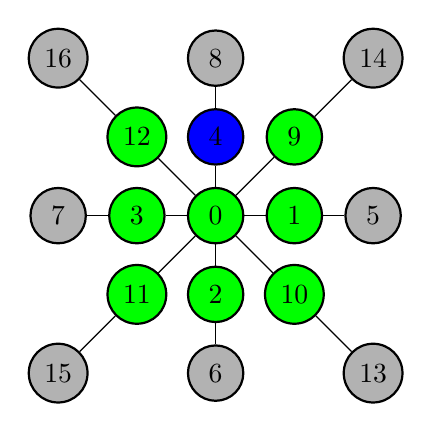
\begin{tikzpicture}
		[node distance={10mm},
		main/.style = {circle, draw, thick, 
                      minimum size=2em}] 
		% Sommets :
		\node[main, fill=green] (0) {$0$}; 
		\node[main, fill=green] (1) [right of=0] {$1$};
		\node[main, fill=green] (2) [below of=0] {$2$};
		\node[main, fill=green] (3) [left of=0] {$3$};
		\node[main, fill=blue] (4) [above of=0] {$4$}; 
		\node[main, fill=black!30!white] (5) [right of=1] {$5$};
		\node[main, fill=black!30!white] (6) [below of=2] {$6$};
		\node[main, fill=black!30!white] (7) [left of=3] {$7$};
		\node[main, fill=black!30!white] (8) [above of=4] {$8$};
		\node[main, fill=green] (9) [right of=4] {$9$};
		\node[main, fill=green] (10) [right of=2] {$10$};
		\node[main, fill=green] (11) [left of=2] {$11$};
		\node[main, fill=green] (12) [left of=4] {$12$};
		\node[main, fill=black!30!white] (13) [right of=6, xshift=10mm] {$13$};
		\node[main, fill=black!30!white] (14) [right of=8, xshift=10mm] {$14$};
		\node[main, fill=black!30!white] (15) [left of=6, xshift=-10mm] {$15$};
		\node[main, fill=black!30!white] (16) [left of=8, xshift=-10mm] {$16$};
		% Arêtes
		\draw (0) -- (1);
		\draw (0) -- (10);
		\draw (0) -- (2);
		\draw (0) -- (11);
		\draw (0) -- (3);
		\draw (0) -- (12);
		\draw (0) -- (4);
		\draw (0) -- (9);

		\draw (1) -- (5);
		\draw (10) -- (13);
		\draw (4) -- (8);
		\draw (9) -- (14);
		\draw (2) -- (6);
		\draw (11) -- (15);
		\draw (3) -- (7);
		\draw (12) -- (16);
		\end{tikzpicture}
	\end{center}
	On a un parcours partiel possible $L_9 = [0, 4, 9, 1, 10, 2, 11, 3, 12]$. Cette fois, $0$ est fermé. On va donc choisir le sommet ouvert le plus ancien, qui est $4$. Son unique successeur non visité est $8$, qui sera donc le prochain sommet visité. Ce processus recommence jusqu'à visiter tous les sommets du graphe.

	\textbf{Conclusion sur le parcours en largeur :} le parcours va visiter les sommets dans l'ordre de découverte. À l'inverse du parcours en profondeur, le parcours en largeur traite tous les voisins\footnote{D'un coup \textit{large}, disons\dots} d'un sommet avant de passer à chacun de ses voisins et de faire de même. On appelle aussi le parcours en largeur le parcours en ``pelure d'oignon'' car on parcours les sommets par couche, comme les pelures d'un oignon.
\subsubsection{Algorithmes}
L'entrée de chacun des algorithmes de parcours est :
\begin{itemize}
	\item Un graphe $G = (S, A)$
	\item Un sommet de départ $s_0$ qui est le premier sommet du parcours $L$
\end{itemize}
La sortie est simplement la liste de parcours.

La question la plus importante qui ressort pour chacun des algorithmes est la manière de stocker les sommets découverts et de choisir quel sommet découvert visiter. On suit les intuitions\footnote{Démontrables formellement.} suivantes :
\begin{itemize}
	\item pour un parcours profondeur, le sommet choisi est celui découvert le plus récemment puisqu'il est successeur de l'ouvert le plus récent.
	\item pour un parcours largeur, le sommet choisi est celui découvert il y a le plus longtemps, puisqu'il est successeur de l'ouvert le plus ancien.
\end{itemize}
Il s'agit respectivement d'un structure $FIFO$ (\textit{First In First Out}) caractéristique du type abstrait \textit{Pile} et d'une structure $LIFO$ (\textit{Last In First Out}) caractéristique du type abstrait \textit{File}.

En stockant les sommets découverts dans un objet d'un de ces types, avec une même structure d'algorithme on obtiendra soit un parcours en profondeur (avec une \textit{Pile}) soit un parcours en largeur (avec une \textit{File}).

\begin{algorithm}
\caption{Parcours en profondeur}\label{alg:graph_dfs}
\KwIn{$Graphe:G = (S, A)$, $Sommet:s_0\in S$}
$\textit{Tableau\textless Booleen\textgreater }:sommets\_visites\left[|S|\right]$\;
\ForAll{$i\in S$}{
	$sommets\_visites[i] = \textit{Faux}$\;
}
$\textit{Liste\textless Sommet\textgreater }:parcours \leftarrow creer\_liste\_vide()$\;
$\textit{Pile\textless Sommet\textgreater }:decouverts\leftarrow creer\_pile\_vide()$\;
$decouverts \leftarrow empiler(decouverts, s_0)$\;
\While {$\neg est\_vide(decouverts)$} {
	$Sommet:u\leftarrow depiler(decouverts)$\;
	\If {$sommets\_visites[u] = \textit{Faux}$} {
		$sommets\_visites[u] = \textit{Vrai}$\;
		$parcours\leftarrow inserer\_en\_queue(parcours, u)$\;
		\ForAll {$v\in succ(G, u)$} {
			$decouverts\leftarrow empiler(decouverts, v)$\;
		}
	}
}
\Return $parcours$\;
\end{algorithm}
\begin{algorithm}
\caption{Parcours en largeur}\label{alg:graph_bfs}
\KwIn{$Graphe:G = (S, A)$, $Sommet:s_0\in S$}
$\textit{Tableau\textless Booleen\textgreater }:sommets\_visites\left[|S|\right]$\;
\ForAll{$i\in S$}{
	$sommets\_visites[i] = \textit{Faux}$\;
}
$\textit{Liste\textless Sommet\textgreater }:parcours \leftarrow creer\_liste\_vide()$\;
$\textit{File\textless Sommet\textgreater }:decouverts\leftarrow creer\_file\_vide()$\;
$decouverts \leftarrow enfiler(decouverts, s_0)$\;
\While {$\neg est\_vide(decouverts)$} {
	$Sommet:u\leftarrow defiler(decouverts)$\;
	\If {$sommets\_visites[u] = \textit{Faux}$} {
		$sommets\_visites[u] = \textit{Vrai}$\;
		$parcours\leftarrow inserer\_en\_queue(parcours, u)$\;
		\ForAll {$v\in succ(G, u)$} {
			$decouverts\leftarrow enfiler(decouverts, v)$\;
		}
	}
}
\Return $parcours$\;
\end{algorithm}

Il s'agit simplement d'empiler/enfiler d'abord le sommet de départ $s_0$ puis boucler le défilement/dépilement du sommet découvert choisi (selon la structure) et de ce sommet maintenant visité, d'empiler/enfiler ses successeurs (qui sont à présent découverts). Si un sommet a déjà été visité, on l'ignore simplement.
\subsection{Algorithme de Roy-Warshall}
L'algorithme de Roy-Warshall\footnote{Comme pointé par Jean Goubault-Larrecq \cite{ENSGraphes}, \textit{Roy} se prononce \textit{roi}. Bernard Roy est français.} permet de calculer la matrice d'accessibilité d'un graphe, c'est-à-dire la matrice $$M\in\mathcal{M}_{|S|}(\mathcal{B})$$ telle que :
$$\forall u, v\in S, M_{u, v} = \left\{
\begin{array}{lcll}
\textit{Vrai} & \text{si} & u\rightarrow^* v & \text{(il existe un chemin de $u$ à $v$)} \\
\textit{Faux} & \text{si} & u\not\rightarrow^*v & \text{(il n'existe pas de chemin de $u$ à $v$)}
\end{array}\right.
$$
C'est la matrice dénotant la clôture réflexive-transitive $\rightarrow^*$.

Cet algorithme est assez classique mais est en fait bien moins rapide \textit{pour la simple détermination de la matrice d'accessibilité} que d'autres algorithmes comme l'algorithme de Tarjan\footnote{L'algorithme de Tarjan sert à déterminer les composantes fortement connexes d'un graphe. Il est de même classe de complexité que l'algorithme de Kosaraju, mais ses constantes sont bien plus faibles. Les composantes fortement connexes d'un graphe induise facilement sa matrice d'accessibilité. On ne présente par ici l'algorithme de Tarjan car il nécessite l'introduction de la notion de \textit{points d'attache}, qui est technique et relativement difficile à expliquer clairement sans passer par 10 pages de démonstrations. Peut-être que ce sera ajouté, mais quand la motivation et une idée d'explication claire seront là.}. Toutefois, l'algorithme de Roy-Warshall peut être facilement généralisé aux graphes valués sans perte d'efficacité. Il reste donc incontournable.

\begin{algorithm}
\caption{Algorithme de Roy-Warshall}\label{alg:roy_warshall}
\KwIn{$Matrice:M_G$, $Entier:n$}
$Matrice:A\leftarrow copie(M_G)$\;
\lForAll {$i\in \{1, \dots, n\}$} {
	$A[i][i] = 1$
}
\ForAll {$k\in [1, \dots, n]$} {
	\ForAll {$i\in[1, \dots, n]$} {
		\ForAll {$j\in[1, \dots, n]$} {
			$A[i][j]\leftarrow A[i][j]\vee (A[i][k] \wedge A[k][j])$\;
		}
	}
}
\Return $A$\;
\end{algorithm}

La complexité temporelle de l'algorithme est visiblement une fonction de $\Theta(n^3)$. \newline
L'algorithme mérite quelques explications, pour justifier qu'il soit correct et ne soit pas simplement le résultat étrange d'une quelconque magie.

\textbf{Notation dans cette section :} Soit $G = (S, A)$ un graphee avec $S = \{1, \dots, n\}$. Pour tout $k\in S$, on note $G_k$ le graphe $(S, A_k)$ où $A_k$ est l'ensemble des couples $(u, v)\in S^2$ telles qu'il existe $u = x_0\rightarrow x_1 \rightarrow \dots \rightarrow x_{l-1} \rightarrow x_l = v$, où $l\in\mathbb{N}$ et pour tout $0\leq i\leq l$, $x_i\in\{1, \dots, k\}$. L'intérieur du chemin est alors $\{x_1, \dots, x_{l-1}\}$ si $l\geq 2$, et $\emptyset$ si $l = 0$.

Autrement dit, c'est le graphe $G$ auquel on ajoute des arcs qui représentent l'existence d'un chemin fait de sommets de $\{1, \dots, k\}$. La matrice de $G_n$ donne l'existence des chemins faits de sommets de $S$. C'est donc la matrice d'accessibilité de $G$.

On veut justifier pourquoi l'algorithme de Roy-Warshall calcule effectivement les matrices de $G_1$ à $G_n$. 

\proposition{Construction par récurrence} Soit $G = (S, A)$. Pour tout $(u, v)\in S^2$, on a :
\begin{enumerate}
	\item $(u, v)\in A_0\Leftrightarrow u = v\vee (u, v)\in A$
	\item $\forall k\in\{1, \dots, n\}, (u, v)\in A_k \Leftrightarrow (u, v)\in A_{k-1}\vee ((u, k)\in A_{k-1}\wedge (k, v)\in A_{k-1})$
\end{enumerate}
\textbf{Signification de la réccurence :} Le deuxième point signifie littéralement : si deux sommets de $G$ sont reliés par un chemin constitué de sommets (qu'on peut supposer tous différents si il n'y a pas de boucle) dans $\{1, \dots, k\}$, c'est que :
\begin{itemize}
	\item si le sommet $k$ n'est pas dans le chemin, ils sont reliés par un chemin de constitué de sommets dans $\{1, \dots, k-1\}$
	\item si le sommet $k$ est dans le chemin, on peut le décomposer en deux moitiés de chemin pour lesquelles $k$ ne sera qu'à une extrêmité mais pas au milieu
\end{itemize}
\textbf{Démonstration :}
\begin{enumerate}
	\item Voir la définition
	\item La réciproque est immédiate car $A_{k-1}\subset A_k$. Si $(u, v)\in A_k$, il existe donc un chemin d'intérieur inclu dans $\{1, \dots, k\}$. D'après le lemme de König, il existe un chemin minimal (donc élémentaire) $\gamma$ entre $u$ et $v$. \newline
	On procède ensuite par disjonction de cas selon que $k$ est ou non dans $\gamma$ :
	\begin{itemize}
		\item Supposons donc que $k$ soit un sommet de $\gamma$. Le sous-chemin de $u$ à $k$ dans $\gamma$ est, comme $\gamma$, à sommets dans $\{1, \dots, k\}$. Or $\gamma$ est élémentaire, donc les sommets du sous-chemin sont dans $\{1, \dots, k-1\}$. Donc $(u, k)\in A_{k-1}$. Par le même raisonnement, on a $(k, v)\in A_{k-1}$
		\item Si $k$ n'est pas un sommet de $\gamma$, alors on a $(u, v)\in A_{k-1}$
	\end{itemize}
\end{enumerate}
L'algorithme de Roy-Warshall trouve là un début de justification. Les lignes 1 et 2 calculent $A_0$ et la triple boucle imbriquée applique la récurrence de la proposition précédente.

Un point chiffonne encore : dans la récurrence de la proposition ci-dessus, $A_k$ est stocké indépendamment de $A_{k-1}$. Dans l'algorithme \ref{alg:roy_warshall}, il n'y a pas de copie de $G_k$ (qui ralentirait considérablement l'algorithme). Tout est fait dans le même tableau, et certaines données pourraient donc s'entrecouper lors des calculs et fausser le résultat. Il faut s'assurer que cela n'arrive pas.

\lemma{} On va avoir besoin pour démontrer la proposition suivante de deux points :\newline
Pour tous $i, j, k\in\{1, \dots, n\}$,
\begin{enumerate}
	\item $(i, k)\in A_{k-1}\Leftrightarrow (i, k)\in A_k$
	\item $(k, j)\in A_{k-1}\Leftrightarrow (k, j)\in A_k$
\end{enumerate}
\textbf{Démonstration :} $\Rightarrow$ est direct car $A_{k-1}\subset A_k$. Si $(i, k)\in A_k$ (resp. $(k, j)$), il existe un chemin minimal donc élémentaire (lemme de König) entre $i$ et $k$ (resp. $j$ et $k$) d'intérieur inclu dans $\{1, \dots, k\}$ et par élémentarité, $k$ n'apparaît pas, donc intérieur inclu dans $\{1, \dots, k-1\}$. D'où $(i, k)\in A_{k-1}$ (resp. $(k, j)\in A_{k-1}$).

\proposition{Correction de l'algorithme de Roy-Warshall} L'algorithme de Roy-Warshall est correct, c'est-à-dire que $A_0$ est correct et les invariants suivants sont vrais pour tout $k\in \{1, \dots, n\}$ :
\newline
Pour tous $i, j\in \{1, \dots, n\}$
\begin{itemize}
	\item pour tout $(u, v)\in \{1, \dots, n\}^2$, $(u, v)\leq_{lex} (i, j) \Rightarrow A[u][v] = (u, v)\in A_k$
	\item pour tout $(u, v)\in \{1, \dots, n\}^2$, $(u, v) >_{lex} (i, j) \Rightarrow A[u][v] = (u, v)\in A_{k-1}$
\end{itemize}
\textbf{Démonstration :} on procède par récurrence

\underline{Initialisation} : pour $k = 0$, le programme est correct par le point 1 de la \refproposition{Construction par récurrence}

\underline{Hérédité} : soit $k\in\{1, \dots, n\}$, soient $(i, j), (u, v)\in\{1, \dots, n\}^2$. Supposons les invariants vrais.
\begin{itemize}
	\item Si $(u, v)\leq_{lex} (i, j)$, par HR, $A[u][v] = (u, v)\in A_{k-1}$.\newline
	D'après le lemme précédent, $A[u][k]$ et $A[k][v]$ sont égalements correctes car les couples $(u, k)$ et $(k, v)$ appartiennent soit à $A_{k-1}$ soit à $A_k$ (la valeur dans la matrice est identique par équivalence des deux appartenance).\newline
	D'où, d'après la proposition ci-dessus, $A[u][v]\vee (A[u][k] \wedge A[k][v]) = (u, v)\in A_k$
	\item Si $(u, v)>_{lex} (i, j)$, le raisonnement est le même.
\end{itemize}

\underline{Conclusion} : L'hypothèse de récurrence est initialisée et héréditaire. Donc le programme calcule bien les $G_k$. À la fin de l'exécution, $G_n$ est le graphe d'accessibilité de $G$.
\subsection{Exercices}
\exercise{Limite de la représentation matricielle}{3} Supposons un cas d'application réel des graphes, comme par exemple la représentation des connexions entre les différents serveurs d'Internet, ou le réseau routier en France, qui relie les différentes villes. Dans chaque cas, on a \textit{au moins} $10^6$ serveurs/villes. Que dire de la réalisabilité \textit{pratique} d'une représentation par matrice d'adjacence d'un tel graphe ?

\exercise{Représentation et implantation}{28} 
\begin{enumerate}
	\item Implanter en C les enregistrements \mintinline{c}{struct MatrixGraph {...};} et \mintinline{c}{struct ListGraph {...};} contenant :
	\begin{itemize}
		\item l'ordre du graphe
		\item la représentation du graphe, soit par matrice d'adjacence (tableau de tableaux), soit par listes d'adjacence (tableau de listes)
	\end{itemize}
	\item Implanter la signature donné à la sous-section \ref{sub:signature_du_type_abstrait_graphe}\footnote{Les identifiants dans le code sont en anglais, toujours.}
	\item Justifier la complexité temporelle dans le pire cas de chaque routine de manipulation
	\item Implanter deux fonctions \mintinline{c}{struct MatrixGraph listgraph_to_matrixgraph(struct ListGraph g);} et \mintinline{c}{struct ListGraph matrixgraph_to_listgraph(struct MatrixGraph g);} qui effectuent une copie d'un graphe en modifiant la représentation utilisée. Quelle est la complexité temporelle de chaque fonction dans le pire cas ?
\end{enumerate}
\exercise{Aiguilles hors d'oignons sans profondeur}{6} Finir l'exécution des algorithmes de parcours en profondeur et en largeur sur le graphe d'exemple donné.

\exercise{Les parcours}{23}
\begin{enumerate}
	\item Quelle est la complexité temporelle des deux parcours dans le pire cas si on choisit de représenter le graphe par matrice d'adjacence ?
	\item Quelle est la complexité temporelle des deux parcours dans le pire cas si on choisit de représenter le graphe par listes d'adjacence ?
	\item Implanter les parcours en profondeur et en largeur avec une représentation du graphe permettant une complexité temporelle optimale.
\end{enumerate}

\exercise{Bicoloriage}{15} On dit qu'un graphe $G = (S, A)$ \textit{non orienté} est \textit{bicoloriable} si il est possible de colorier par une fonction $C:S\rightarrow \mathcal{B}$ chacun de ses sommets avec deux couleurs $0$ et $1$ de sorte que pour chaque arête $\{a, b\}\in A$, $C(a)\neq C(b)$.
\begin{enumerate}
	\item Justifier que $G$ est bicoloriable \textit{ssi} chacune de ses componentes connexes est bicoloriable
	\item Montrer qu'un graphe $G$ connexe non orienté est bicoloriable \textit{ssi} pour tout sommet $u$ visité lors d'un parcours, pour tout $v\in succ(u)$, $C(u)\neq C(v)$ 
	\item En déduire une fonction \mintinline{c}{bool graph_is_2coloriable(Graph g);} \newline
	\textit{\underline{Remarque :} On n'impose pas la représentation du graphe, qui est au choix du lecteur, mais influe sur la réponse à la question suivante.}
	\item Quelle est sa classe de complexité temporelle ?
\end{enumerate}

\exercise{Plus court chemin}{15}

\exercise{Labyrinthe}{} On s'intéresse à la génération et à l'exploration de labyrinthes parfaits.

\exercise{Arbres et graphes}{24} On s'intéresse dans cet exercice à la relation entre les arbres et les graphes.
\definition{Arbre non orienté} {
	En théorie des graphes, un \textit{arbre non orienté} est un graphe non orienté connexe acyclique.
}
\begin{enumerate}
	\item Justifier que cette définition contient celle donnée à la section \ref{sec:arbres_binaires}.
	\item Montrer que les propriétés suivantes sont toutes équivalentes pour $G = (S, A)$ un graphe non orienté :
	\begin{enumerate}
		\item $G$ est un arbre non orienté
		\item $G$ est connexe et a $(n-1)$ arêtes
		\item $G$ est acyclique et a $(n-1)$ arêtes
		\item Pour tous $x, y\in S$, il existe une unique chaîne entre $x$ et $y$
		\item $G$ est connexe minimal, c'est-à-dire que $G$ est connexe et la suppression d'une arête de $G$ détruit la connexité.
		\item $G$ est acyclique maximal, c'est-à-dire que $G$ est acyclique et ajouter une arête à $G$ crée un cycle.
	\end{enumerate}
	On en déduit la définition :
\definition{Arbre couvrant} {
	Soit $G = (S, A)$ un graphe connexe \textit{non orienté}. Un \textit{arbre couvrant} de $G$ est un sous-graphe de $G$ connexe minimal dont les sommets sont ceux de $G$.
}\vspace*{5mm}
	\item Quel algorithme du cours permet de calculer un arbre couvrant de $G$ ?
\end{enumerate}
\end{document}